\documentclass[a4paper, 12pt]{article}

\usepackage[T1]{fontenc}
\usepackage[polish]{babel} 
\usepackage[utf8]{inputenc} 
\let\lll\undefined
\usepackage{setspace}
\usepackage{fancyhdr}
\usepackage{hyperref}
\usepackage{pdfpages}
\usepackage{listings}
\usepackage{color}
\usepackage{graphicx}
\usepackage{enumitem}
\usepackage{latexsym}
\usepackage[3D]{movie15}
\usepackage{hyperref}
\pagestyle{fancy} 
\hypersetup{
    colorlinks=true,
    linkcolor=blue,
    filecolor=magenta,      
    urlcolor=cyan,
}
\newcommand{\mainmatter}{\clearpage \cfoot{\thepage\ of \pageref{LastPage}}
\pagenumbering{arabic}} 
\lstset{language=bash}  
\begin{document}

	\begin{titlepage}

\includegraphics[width = 40mm]{logo.jpg}
		\begin{center}
    			\vspace{3cm}
    					\Large\textit{\textbf{Rozproszony algorytm genetyczny  do wyszukiwania globalnej ekstremy: MPI}}
    					\Large\textit{\textbf{Programowanie równoległe i rozproszone}}
   			\vspace{4cm}
		\end{center} 

		\hfill\begin{minipage}{0.54\textwidth}
			\Large Wykonanie:\newline
				1. Ivan Prakapets  \newline
				2. Piotr Jeleniewicz 
		\vspace{\baselineskip}
		\end{minipage}
		
		\hfill\begin{minipage}{0.54\textwidth}
			\Large Sprawdzająca:\newline
		 		dr inż. Zuzanna Krawczyk
\vspace{\baselineskip}
		\end{minipage}
	
		\hfill\begin{minipage}{0.7\textwidth}
		\vspace{1cm}
			\Large Warszawa, 2020
			\vspace{\baselineskip}
		\end{minipage}
	\end{titlepage}
\newpage
\mainmatter
\setlength{\headheight}{15pt}
\doublespacing
\tableofcontents
\newpage

\linespread{0.5}
\setlist{nolistsep}

\section{Opis uruchomienia i wywołania programu}
Aby uruchomić program i otworzyć GUI trzeba wpisać komendę: \texttt{python3 main.py} lub poprzez IDE np. PyCharm.

Po uruchomieniu programu i otworzeniu ustawienia-GUI z kilkoma polami:
\begin{itemize}
    \item f(x, y) input string
    \item chromosomes
    \item generations number input string liczba pokoleń
    \item optimizer function (min or max) funkcja optymalizatora (min lub max)
\end{itemize}
Oraz pola z ptaszkami (funkcjonalne):
\begin{itemize}
    \item mutation - dodanie mutacji do każdej części (4 osobników) nowego pokolenia
    \item show statistics - pokazuje dokładne informacje o każdym pokoleniu
    \item save all files - zapisuje do folderu results statystyki wyników z animacją w .gif oraz ga-statystyki + do folderu generations dane csv z kolumnami x, y, f (x, y)
    \item show plot - pokazuje animację ewaluacji
    
\end{itemize}


\section{Dokładny opis realizacji problemu}
\paragraph{Opis programu} \hfill \break
Program w przybliżeniu oblicza minimum lub maksimum funkcji o dwóch parametrach na podstawie algorytmu genetycznego.
Każdy osobnik ma jedną  \texttt{chromosom (x, y)} i ze względu na to, że osobnik i chromosom mają to samo znaczenie, pokolenie składa się z części, gdzie jedna część to 4 osobniki, w konsekwencji liczba chromosomów jest wielokrotnością 4.

Zasada crossover to:\\
(x\_better, y\_best), (y\_better, y\_best), (x\_best, y\_better), (x\_best, y\_good)

gdzie (x\_best, y\_best), (x\_better, y\_better), (x\_good, y\_good) są zaznaczonymi individs.

\paragraph{Funkcji genetyczne i rozwiązanie algorytmiczne.} \hfill \break
W tej chwili w programie realizowany jest genetyczne algorytm, który jest parametryzowany przez Dane wejściowe za pomocą GUI.

Pojedynczy osobnik przenosi w każdym swoim genie informacje o odpowiedniej współrzędnej X lub Y. Populacja jest określana przez wiele osobników, ale populacja jest podzielona na 4 osobniki. To rozwiązanie jest spowodowane próbą uniknięcia zbieżności do lokalnego optimum, ponieważ jest to zadanie o znalezieniu globalnego ekstremum. Taki podział, w wielu przypadkach nie pozwala zdominować jednego genotypu w całej populacji, ale wręcz przeciwnie, daje \textbf{ewolucję} większą dynamikę. Dla każdej takiej części populacji stosuje się następujący algorytm:
\begin{enumerate}
    \item Selekcja jest podobna do metody rankingowej. Wybiera się 3 osobniki o najlepszych wskaźnikach funkcji fitness (tzn. dokonuje się sortowania osobników w kolejności rosnącej/malejącej określonej przez użytkownika funkcji),
    \item Następnie stosuje się funkcję krzyżowania w taki sposób, że nowa generacja (dokładniej nowy segment populacji 4 osobników) otrzymuje 2 pary niezmutowanych genów od osobnika o lepszym odczycie funkcji fitness i po parze zmutowanych genów od pozostałych dwóch osobników. 
\end{enumerate}

Zasada selekcji, krzyżowania i mutacji wyraźnie wygląda tak (w generacji N chromosomów osobników są już posortowane w odpowiedniej kolejności, a mały czarny kwadrat oznacza mutację):\\
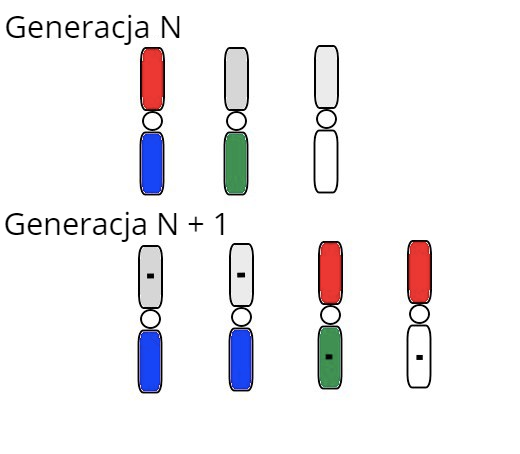
\includegraphics[scale=3]{generacji.png}\\
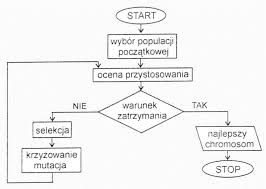
\includegraphics[scale=0.92]{schemat.jpg}
\section{Testy programu pokazujące np. uzyskane przyspieszenie}
\paragraph{Funkcja 1} \hfill \break
\[
f(x, y) = sin(x) + cos(y)
\]
\paragraph{Funkcja 2} \hfill \break
\[
    \frac{4 \sqrt{x} - 5y}{ 3x ^ 2 + 2 y ^ 2 - 2 x + 1}
\]
\paragraph{Funkcja 3} \hfill \break
\[
f(x, y) = sinx
\]

\paragraph{Funkcja 4}
\[
f(x, y) = 4exp(-x^2 - y^2)
%5exp(-(x - 3)^2 - (y - 3)^2)
\]
\[
f(x, y) = (\sqrt{x}- 5y ) / (x^2+ y^2  - 2x + 10)
\]

\section{Wnioski} 

\begin{enumerate}
    \item Właściwy zestaw parametrów pozwala na dość dokładne znalezienie globalnego ekstremum funkcji z dwóch zmiennych
    \item Wizualizacja może pomóc w debugowaniu i ulepszaniu algorytmu, a także pomaga zrozumieć przebieg i zasady samego algorytmu genetycznego
    \item Udało nam się poprawnie zrównoleglić algorytm genetyczny i odpowiednio dobrać
parametry aby osiągnąć przyśpieszenie
\end{enumerate}
\label{LastPage}~
\label{LastPageOfBackMatter}~		
\end{document}